\subsection{Modelo insumo-produto e contas de emissões}
\label{sec:derivacao}
\label{sec:atribuicoes}

Na notação adotada, letras minúsculas sem índices representam vetores-coluna com 67 componentes, e letras maiúsculas representam matrizes $67\times67$. O chapéu indica a matriz diagonal formada pelos elementos de um vetor.

A MIP descreve o fornecimento de insumos entre atividades e o atendimento à demanda final. Dela obtêm-se os vetores de produção bruta $x$ e de demanda final $y$, além da inversa de Leontief $L$. A produção bruta atende aos usos intermediários e à demanda final. Sob coeficientes técnicos fixos, cada elemento $L_{ij}$ representa a produção da atividade $i$ necessária por unidade monetária de demanda final dos produtos da atividade $j$, incluindo requisitos diretos e indiretos \parencite{millerBlair2009}.

O vetor $\varphi$ contém os coeficientes de emissão interpolados de \textcite{sanguinetAzzoni2024}, e $\widehat{\varphi}$ é a matriz diagonal desses coeficientes.

Para relacionar as atividades emissoras aos produtos finais, define-se a matriz de atribuição de emissões:
\begin{equation}
F=\widehat{\varphi}L\widehat y,\qquad F_{ij}=\varphi_iL_{ij}y_j.
\label{eq:matriz-atribuicao}
\end{equation}
Cada $F_{ij}$ representa as emissões da atividade $i$ atribuídas à demanda final dos produtos da atividade $j$, incluindo requisitos diretos e indiretos, em Gg de CO\textsubscript{2}.

A soma de cada linha de $F$ mantém a atividade em que a emissão ocorre e fornece a conta pela produção, $c$; a soma de cada coluna reúne as emissões atribuídas aos produtos finais de uma atividade e fornece a conta pela demanda, $u$ \parencite{marques2012}:
\begin{align}
c_i&=\sum_jF_{ij}=\varphi_i x_i, & c&=F\mathbf{1}=\widehat{\varphi}x,
\label{eq:conta-producao}
\\
u_j&=\sum_iF_{ij}=y_j\sum_i\varphi_iL_{ij}, & u&=F^\top\mathbf{1}.
\label{eq:conta-demanda}
\end{align}
Aqui, $\mathbf{1}$ é o vetor de uns e $\top$ indica transposição. As contas preservam o mesmo total de emissões, $\mathbf{1}^\top c=\mathbf{1}^\top F\mathbf{1}=\mathbf{1}^\top u$, embora sua distribuição entre as atividades possa diferir. A Figura~\ref{fig:exemplo-atribuicoes} ilustra as duas formas de atribuição em uma economia hipotética com quatro setores.

% Figura vetorial copiada sem edição de:
% C:/GitHub/Mestrado/0-Projeto de Dissertação/figura_economia/contabilidade_com_sankey.pdf
% SHA-256: 861F8B5C1FDEBE3C96B31D8BD96763C2829FA2AE72703160C83949E4ACD6BF29
\begin{figure}[!htbp]
\centering
\caption{Atribuição das emissões pela produção e pela demanda em uma economia ilustrativa.}
\label{fig:exemplo-atribuicoes}
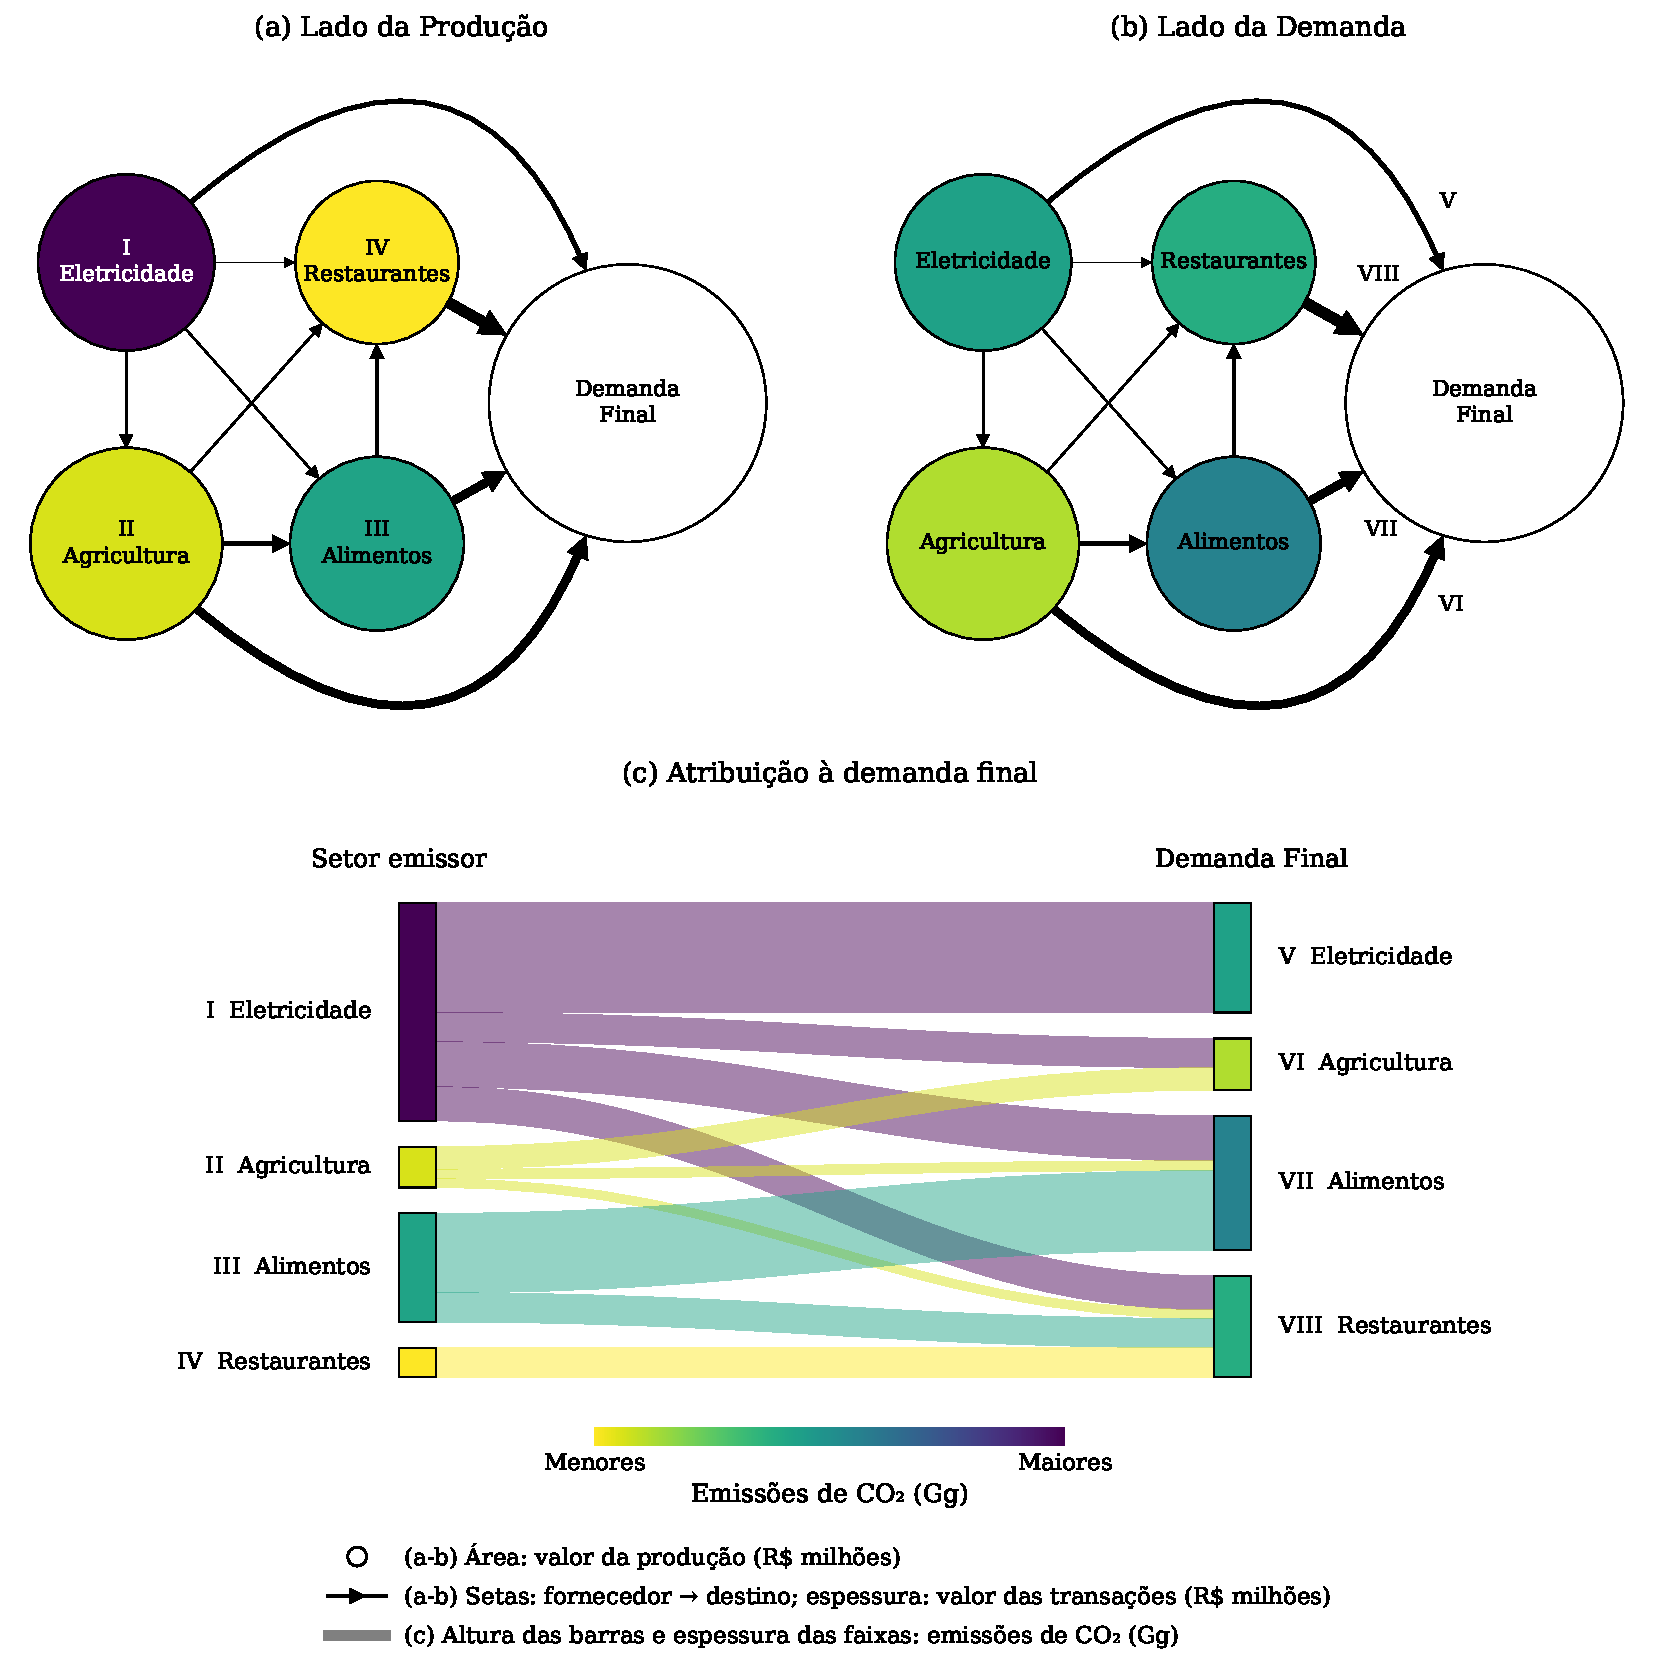
\includegraphics[width=\textwidth,height=0.76\textheight,keepaspectratio]{figuras/atribuicao_cadeia_alimentos.pdf}
\begin{notas}
Nota: Exemplo de atribuição de emissões pela ótica da produção e da demanda, para uma economia hipotética de 4 setores. Em (a--b), áreas e espessuras das setas expressam valores monetários; no nó Demanda Final, a área indica o valor recebido, incluindo exportações. As cores representam as emissões por setor pela ótica da produção, $c_i$ em (a) e pela ótica da demanda $u_i$ em (b). Em (c), as barras à esquerda representam as origens emissoras (ótica da produção) (I--IV) e as barras à direita, os produtos finais (ótica da demanda) (V--VIII). As alturas das barras e as espessuras das faixas expressam emissões em Gg de CO\textsubscript{2}. Os três quadros compartilham a escala de cores.
\end{notas}
\end{figure}
\clearpage
